\section{Orthogonal functions and orthogonal matrices}
\label{sec:orthogonal-matrices}

\begin{definition}{Isometries and orthogonal maps}{isometry-orthogonal-map}
  Let $V,W$ be real inner product spaces, and let $T:V\to W$ be a
  linear transformation. We say that $T$ is an \textbf{isometry}%
  \index{isometry}%
  \index{linear transformation!isometry} if for all
  $\vect{u},\vect{v}\in V$,
  \begin{equation*}
    \iprod{T(\vect{u}),T(\vect{v})} = \iprod{\vect{u},\vect{v}}.
  \end{equation*}
  Moreover, $T$ is called an \textbf{orthogonal transformation}%
  \index{orthogonal transformation}%
  \index{linear transformation!orthogonal}, or simply
  \textbf{orthogonal}, if it is an isometry and invertible.
\end{definition}

In particular, if $T$ is an isometry, we have
$\norm{T\vect{v}} = \sqrt{\iprod{T\vect{v},T\vect{v}}} =
\sqrt{\iprod{\vect{v},\vect{v}}} = \norm{\vect{v}}$, so isometries
preserve the norm. (This is fact where the name ``isometry'' comes
from: from Greek ``isos'', meaning ``equal'', and ``metron'', meaning
``measure''). Conversely, any norm-preserving linear function is an
isometry, as the following proposition shows.

\begin{proposition}{Norm-preserving linear maps are isometries}{norm-isometry}
  Let $T:V\to W$ be a linear function such that for all
  $\vect{v}\in V$, $\norm{T\vect{v}} = \norm{\vect{v}}$. Then $T$ is
  an isometry.
\end{proposition}

\begin{proof}
  We first note that for all $\vect{u},\vect{v}\in V$,
  \begin{equation*}
    \iprod{\vect{u},\vect{v}}
    ~=~ \frac{1}{2}(\iprod{\vect{u},\vect{v}} + \iprod{\vect{v},\vect{u}})
    ~=~ \frac{1}{2}(\iprod{\vect{u}+\vect{v},\vect{u}+\vect{v}}
    - \iprod{\vect{u},\vect{u}} - \iprod{\vect{v},\vect{v}})
    ~=~ \frac{1}{2}(\norm{\vect{u}+\vect{v}}^2
    - \norm{\vect{u}}^2 - \norm{\vect{v}}^2).
  \end{equation*}
  Now suppose $T$ is norm-preserving and linear. Then for all
  $\vect{u},\vect{v}\in V$,
  \begin{eqnarray*}
    \iprod{T(\vect{u}),T(\vect{v})}
    &=& \frac{1}{2}(\norm{T(\vect{u})+T(\vect{v})}^2 - \norm{T(\vect{u})}^2 -
        \norm{T(\vect{v})}^2) \\
    &=& \frac{1}{2}(\norm{T(\vect{u}+\vect{v})}^2 - \norm{T(\vect{u})}^2 -
        \norm{T(\vect{v})}^2) \\
    &=& \frac{1}{2}(\norm{\vect{u}+\vect{v}}^2 -
        \norm{\vect{u}}^2 - \norm{\vect{v}^2}) \\
    &=& \iprod{\vect{u},\vect{v}}.
  \end{eqnarray*}
  Therefore, $T$ is an isometry.
\end{proof}

We also note that if $T$ is an isometry and $\vect{u}\orth\vect{v}$,
then $T(\vect{u})\orth T(\vect{v})$, because
$\iprod{T(\vect{u}),T(\vect{v})} = \iprod{\vect{u},\vect{v}} = 0$. So
isometries preserve right angles. In fact, isometries also preserve
arbitrary angles, due to the formula
$\cos\theta =
\frac{\iprod{\vect{u},\vect{v}}}{\norm{\vect{u}}\,\norm{\vect{v}}} =
\frac{\iprod{T(\vect{u}),T(\vect{v})}}
{\norm{T(\vect{u})}\,\norm{T(\vect{v})}}$.

\begin{example}{Orthogonal transformations on $R^n$}{orthogonal-transformation-rn}
  Let $T_1,T_2,T_3:\R^2\to\R^2$ be the linear transformations with matrices
  \begin{equation*}
    \coord{T_1} = \begin{mymatrix}{cc} 0 & -1 \\ 1 & 0 \end{mymatrix},
    \quad
    \coord{T_2} = \begin{mymatrix}{cc} 2 & 0 \\ 0 & 2 \end{mymatrix},
    \quad\mbox{and}\quad
    \coord{T_3} = \begin{mymatrix}{cc} 1 & 1 \\ 0 & 1 \end{mymatrix},
  \end{equation*}
  respectively. $T_1$ is a counterclockwise rotation by $90^{\circ}$,
  $T_2$ is a scaling by a factor of $2$, and $T_3$ is a shearing.
  Then $T_1$ is orthogonal, but $T_2$ and $T_3$ are not. Note that
  $T_1$, being a rotation, preserves lengths and angles. $T_2$
  preserves angles but not lengths. $T_3$ preserves neither lengths
  nor angles.
  \begin{center}
    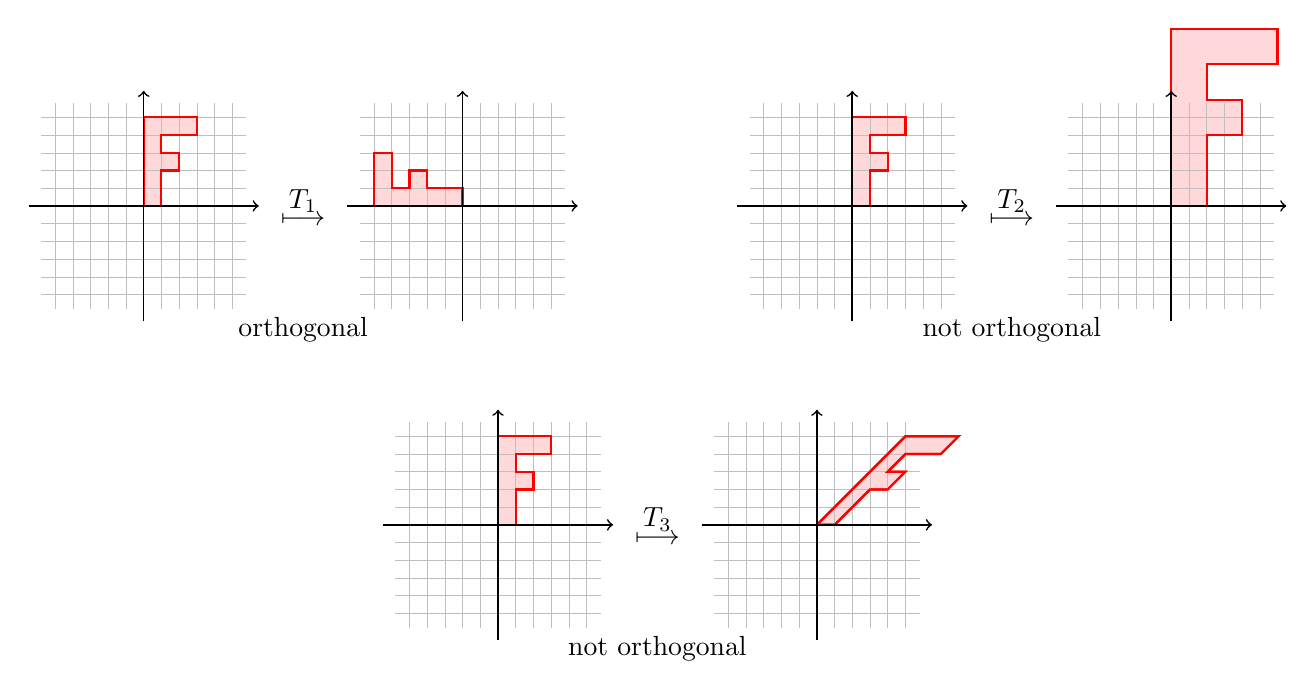
\begin{tikzpicture}[scale=0.9]
      \begin{scope}
        \begin{scope}[scale=0.25]
          \draw[red,thick,fill=red!15]
          (0,0) -- (0,5) -- (3,5) -- (3,4) -- (1,4) --
          (1,3) -- (2,3) -- (2,2) -- (1,2) -- (1,0) -- cycle;
          \draw[step=1cm, gray!50, very thin] (-5.8,-5.8) grid (5.8,5.8);
          \draw[red,thick]
          (0,0) -- (0,5) -- (3,5) -- (3,4) -- (1,4) --
          (1,3) -- (2,3) -- (2,2) -- (1,2) -- (1,0) -- cycle;
          \draw[semithick,->] (-6.5,0) -- (6.5,0);
          \draw[semithick,->] (0,-6.5) -- (0,6.5);
        \end{scope}
        \begin{scope}[xshift=2.25cm]
          \path (0,0) node {$\stackrel{\displaystyle T_1}{\longmapsto}$};
          \path (0,-1.75) node {orthogonal};
        \end{scope}
        \begin{scope}[xshift=4.5cm,scale=0.25]
          \draw[red,thick,fill=red!15,cm={0,1,-1,0,(0,0)}]
          (0,0) -- (0,5) -- (3,5) -- (3,4) -- (1,4) --
          (1,3) -- (2,3) -- (2,2) -- (1,2) -- (1,0) -- cycle;
          \draw[step=1cm, gray!50, very thin] (-5.8,-5.8) grid (5.8,5.8);
          \draw[red,thick,cm={0,1,-1,0,(0,0)}]
          (0,0) -- (0,5) -- (3,5) -- (3,4) -- (1,4) --
          (1,3) -- (2,3) -- (2,2) -- (1,2) -- (1,0) -- cycle;
          \draw[semithick,->] (-6.5,0) -- (6.5,0);
          \draw[semithick,->] (0,-6.5) -- (0,6.5);
        \end{scope}
      \end{scope}
      \begin{scope}[xshift=10cm]
        \begin{scope}[scale=0.25]
          \draw[red,thick,fill=red!15]
          (0,0) -- (0,5) -- (3,5) -- (3,4) -- (1,4) --
          (1,3) -- (2,3) -- (2,2) -- (1,2) -- (1,0) -- cycle;
          \draw[step=1cm, gray!50, very thin] (-5.8,-5.8) grid (5.8,5.8);
          \draw[red,thick]
          (0,0) -- (0,5) -- (3,5) -- (3,4) -- (1,4) --
          (1,3) -- (2,3) -- (2,2) -- (1,2) -- (1,0) -- cycle;
          \draw[semithick,->] (-6.5,0) -- (6.5,0);
          \draw[semithick,->] (0,-6.5) -- (0,6.5);
        \end{scope}
        \begin{scope}[xshift=2.25cm]
          \path (0,0) node {$\stackrel{\displaystyle T_2}{\longmapsto}$};
          \path (0,-1.75) node {not orthogonal};
        \end{scope}
        \begin{scope}[xshift=4.5cm,scale=0.25]
          \draw[red,thick,fill=red!15,cm={2,0,0,2,(0,0)}]
          (0,0) -- (0,5) -- (3,5) -- (3,4) -- (1,4) --
          (1,3) -- (2,3) -- (2,2) -- (1,2) -- (1,0) -- cycle;
          \draw[step=1cm, gray!50, very thin] (-5.8,-5.8) grid (5.8,5.8);
          \draw[red,thick,cm={2,0,0,2,(0,0)}]
          (0,0) -- (0,5) -- (3,5) -- (3,4) -- (1,4) --
          (1,3) -- (2,3) -- (2,2) -- (1,2) -- (1,0) -- cycle;
          \draw[semithick,->] (-6.5,0) -- (6.5,0);
          \draw[semithick,->] (0,-6.5) -- (0,6.5);
        \end{scope}
      \end{scope}
      \begin{scope}[xshift=5cm,yshift=-4.5cm]
        \begin{scope}[scale=0.25]
          \draw[red,thick,fill=red!15]
          (0,0) -- (0,5) -- (3,5) -- (3,4) -- (1,4) --
          (1,3) -- (2,3) -- (2,2) -- (1,2) -- (1,0) -- cycle;
          \draw[step=1cm, gray!50, very thin] (-5.8,-5.8) grid (5.8,5.8);
          \draw[red,thick]
          (0,0) -- (0,5) -- (3,5) -- (3,4) -- (1,4) --
          (1,3) -- (2,3) -- (2,2) -- (1,2) -- (1,0) -- cycle;
          \draw[semithick,->] (-6.5,0) -- (6.5,0);
          \draw[semithick,->] (0,-6.5) -- (0,6.5);
        \end{scope}
        \begin{scope}[xshift=2.25cm]
          \path (0,0) node {$\stackrel{\displaystyle T_3}{\longmapsto}$};
          \path (0,-1.75) node {not orthogonal};
        \end{scope}
        \begin{scope}[xshift=4.5cm,scale=0.25]
          \draw[red,thick,fill=red!15,cm={1,0,1,1,(0,0)}]
          (0,0) -- (0,5) -- (3,5) -- (3,4) -- (1,4) --
          (1,3) -- (2,3) -- (2,2) -- (1,2) -- (1,0) -- cycle;
          \draw[step=1cm, gray!50, very thin] (-5.8,-5.8) grid (5.8,5.8);
          \draw[red,thick,cm={1,0,1,1,(0,0)}]
          (0,0) -- (0,5) -- (3,5) -- (3,4) -- (1,4) --
          (1,3) -- (2,3) -- (2,2) -- (1,2) -- (1,0) -- cycle;
          \draw[semithick,->] (-6.5,0) -- (6.5,0);
          \draw[semithick,->] (0,-6.5) -- (0,6.5);
        \end{scope}
      \end{scope}
    \end{tikzpicture}
  \end{center}
\end{example}

\begin{proposition}{The matrix of an orthogonal transformation}{matrix-orthogonal}
  Let $V,W$ be finite-dimensional real inner product spaces and let
  $T:V\to W$ be a linear transformation. Let $B$ and $C$ be
  orthonormal bases of $V$ and $W$, respectively, and let
  $P=\coord{T}_{C,B}$ be the matrix of $T$ with respect to the bases
  $B$ and $C$. Then
  \begin{enumialphparenastyle}
    \begin{enumerate}
    \item $T$ is an isometry if and only if $P^TP = I$.
    \item $T$ is orthogonal if and only if $P^TP = I$ and $\dim V=\dim
      W$.
    \end{enumerate}
  \end{enumialphparenastyle}
\end{proposition}

\begin{proof}
  (a) Recall from Proposition~\ref{prop:inner-product-dot-product}
  that for all $\vect{u},\vect{v}\in V$, we have
  $\iprod{\vect{u},\vect{v}} = \coord{\vect{u}}_B\dotprod
  \coord{\vect{v}}_B$. Consider two vectors $\vect{u},\vect{v}\in V$
  and let $\vect{t}=\coord{u}_B$ and $\vect{s}=\coord{v}_B$. We have:
  \begin{eqnarray*}
    \iprod{T(\vect{u}),T(\vect{v})} = \iprod{\vect{u},\vect{v}}
    &\iff& \coord{T(\vect{u})}_C\dotprod \coord{T(\vect{v})}_C
           = \coord{\vect{u}}_B\dotprod \coord{\vect{v}}_B \\
    &\iff& (\coord{T}_{C,B}\coord{\vect{u}}_B)\dotprod (\coord{T}_{C,B}\coord{\vect{v}}_B)
           = \coord{\vect{u}}_B\dotprod \coord{\vect{v}}_B \\
    &\iff& (P\vect{t})\dotprod (P\vect{s})
           = \vect{t}\dotprod \vect{s} \\
    &\iff& \vect{t}^T P^T P\vect{s}
           = \vect{t}^T \vect{s} \\
    &\iff& \vect{t}^T P^T P\vect{s}
           = \vect{t}^T I \vect{s}.
  \end{eqnarray*}
  Therefore, $T$ is an isometry if and only if
  $\vect{t}^T P^T P\vect{s} = \vect{t}^T I \vect{s}$ holds for all
  $\vect{t},\vect{s}\in\R^m$. If $P^TP=I$, then this is clearly
  true. Conversely, assume
  $\vect{t}^T P^T P\vect{s} = \vect{t}^T I \vect{s}$ holds for all
  $\vect{t},\vect{s}\in\R^m$. Then by taking $\vect{t}$ and $\vect{s}$
  to be the $i\th$ and $j\th$ standard basis vector, it follows that
  the $(i,j)$-entry of $P^TP$ is equal to the $(i,j)$-entry of $I$,
  for all $i$ and $j$. Therefore, $P^TP=I$.

  (b) By definition, $T$ is orthogonal if and only if it is an
  isometry and invertible. Therefore, if $T$ is orthogonal, then
  $P^TP=I$ by part (a) and $\dim V=\dim W$ because every invertible
  matrix is square (see
  Theorem~\ref{thm:invertible-square}). Conversely, assume that
  $P^TP=I$ and $\dim V=\dim W$. Then $T$ is an isometry by part
  (a). Also, by Theorem~\ref{thm:right-square-left}, since $P$ is
  square and $P^T$ is a left inverse of $P$, the matrix $P$, and
  therefore the linear transformation $T$, is invertible. Therefore,
  $T$ is orthogonal.
\end{proof}

\begin{example}{Orthogonal transformations}{orthogonal-transformations}
  Which of the following matrices define orthogonal transformations?
  Which ones define isometries?
  \begin{equation*}
    A = \begin{mymatrix}{rr}
      0  & 1 \\
      -1 & 0 \\
    \end{mymatrix},\quad
    B = \begin{mymatrix}{rr}
      1 & 1 \\
      1 & 0 \\
    \end{mymatrix},\quad
    C = \frac{1}{\sqrt{2}}\begin{mymatrix}{rr}
      1 & 1 \\
      1 & -1 \\
    \end{mymatrix},\quad
    D = \frac{1}{3}\begin{mymatrix}{rr}
      1 & -2 \\
      2 & -1 \\
      2 &  2 \\
    \end{mymatrix}.
  \end{equation*}
\end{example}

\begin{solution}
  We have
  \begin{equation*}
    A^TA = \begin{mymatrix}{rr}
      0  & 1 \\
      -1 & 0 \\
    \end{mymatrix}\begin{mymatrix}{rr}
      0  & -1 \\
      1 & 0 \\
    \end{mymatrix} = \begin{mymatrix}{rr}
      1 & 0 \\
      0 & 1 \\
    \end{mymatrix} = I,
  \end{equation*}
  and therefore $A$ defines an isometry and (since it is also a square
  matrix) an orthogonal transformation. We have
  \begin{equation*}
    B^TB = \begin{mymatrix}{rr}
      1 & 1 \\
      1 & 0 \\
    \end{mymatrix}\begin{mymatrix}{rr}
      1 & 1 \\
      1 & 0 \\
    \end{mymatrix} = \begin{mymatrix}{rr}
      2 & 1 \\
      1 & 1 \\
    \end{mymatrix} \neq I,
  \end{equation*}
  so the linear transformation defined by $B$ is neither an isometry
  nor orthogonal. A similar pair of calculations shows that $C^TC=I$
  and $D^TD=I$, so both $C$ and $D$ are isometries. Since $C$ is a
  square matrix, it is also orthogonal. $D$ is not a square matrix,
  and therefore not orthogonal.  
\end{solution}

In light of Proposition~\ref{prop:matrix-orthogonal}, we say that an
$n\times n$-matrix $P$ is orthogonal if $P^TP=I$.

\begin{definition}{Orthogonal matrix}{orthogonal-matrix}
  An $n\times n$-matrix $P$ is called \textbf{orthogonal}%
  \index{orthogonal matrix}%
  \index{matrix!orthogonal} if $P^TP=I$.
\end{definition}

The following proposition gives several equivalent ways of checking
whether an $n\times n$-matrix $P$ is orthogonal.

\begin{proposition}{Conditions for orthogonal matrices}{conditions-orthogonal-matrix}
  The following are equivalent for an $n\times n$-matrix $P$:
  \begin{enumialphparenastyle}
    \begin{enumerate}
    \item $P$ is orthogonal.
    \item $P^TP=I$.
    \item $P$ is invertible and $P^{-1}=P^T$.
    \item $PP^T=I$.
    \item $P^T$ is orthogonal.
    \item The columns of $P$ form an orthonormal set of vectors.
    \item The rows of $P$ form an orthonormal set of vectors.
    \end{enumerate}
  \end{enumialphparenastyle}
\end{proposition}

\begin{proof}
  The equivalence (a) {\textiff} (b) is just the definition of
  orthogonality, bearing in mind that $P$ is assumed to be a square
  matrix. The equivalences (b) {\textiff} (c) {\textiff} (d) follow
  from Theorem~\ref{thm:right-square-left}, since a square matrix is
  invertible if and only if it is left invertible if and only if it is
  right invertible.  The equivalence (d) {\textiff} (e) is again just
  the definition of orthogonality, this time applied to $P^T$. To show
  (b) {\textiff} (f), let $\vect{a}_1,\ldots,\vect{a}_n$ be the
  columns of $P$, and let $\vect{e}_1,\ldots,\vect{e}_n$ be the
  standard basis vectors of $\R^n$. Then we have $P^TP = I$ if and
  only if for all $i,j$, the $(i,j)$-entry of $P^TP$ is equal to the
  $(i,j)$-entry of $I$.  But the $(i,j)$-entry of $P^TP$ is
  $\vect{e}_i^TP^TP\vect{e}_j = \vect{a}_i^T\vect{a}_j =
  \vect{a}_i\dotprod\vect{a}_j$. On the other hand, the $(i,j)$-entry
  of $I$ is $1$ if $i=j$ and $0$ if $i\neq j$. It follows that
  $P^TP=I$ if and only if for all $i,j$,
  \begin{equation*}
    \vect{a}_i\dotprod\vect{a}_j=\begin{cases}
      1 & \mbox{when $i=j$ and} \\
      0 & \mbox{otherwise}.
    \end{cases}
  \end{equation*}
  But this is exactly what it means for $\vect{a}_1,\ldots,\vect{a}_n$
  to form an orthonormal set.
  The proof of (d) {\textiff} (g) is completely analogous, using rows
  instead of columns.
\end{proof}

\begin{example}{Orthogonal matrices}{conditions-orthogonal-matrix}
  Determine which of the following matrices are orthogonal by checking
  whether the columns form an orthonormal set.
  \begin{equation*}
    A = \begin{mymatrix}{rrr}
      0 & -1 & 0 \\
      1 & 0 & 0 \\
      0 & 0 & 1 \\
    \end{mymatrix},
    \quad
    B = \frac{1}{3}
    \begin{mymatrix}{rrr}
      2  & -1 &  2 \\
      -1 &  2 &  2 \\
      2  &  2 & -1 \\
    \end{mymatrix},
    \quad
    C = 
    \begin{mymatrix}{rrr}
      3 &  4 & 0 \\
      4 & -3 & 0 \\
      0 &  0 & 5 \\
    \end{mymatrix},
    \quad
    D = \frac{1}{3}
    \begin{mymatrix}{rrr}
      2  &  1 &  2 \\
      1  &  2 &  2 \\
      2  &  2 &  1 \\
    \end{mymatrix}.
  \end{equation*}
\end{example}

\begin{solution}
  By Proposition~\ref{prop:conditions-orthogonal-matrix}, it suffices to check
  whether the columns of each matrix are orthonormal. This is the case
  for $A$ and $B$. For example, the columns of $B$ are
  \begin{equation*}
    \vect{b}_1 = \frac{1}{3}\begin{mymatrix}{r} 2 \\ -1 \\ 2 \end{mymatrix},
    \quad
    \vect{b}_2 = \frac{1}{3}\begin{mymatrix}{r} -1 \\ 2 \\ 2 \end{mymatrix},
    \quad\mbox{and}\quad
    \vect{b}_3 = \frac{1}{3}\begin{mymatrix}{r} 2 \\ 2 \\ -1 \end{mymatrix},
  \end{equation*}
  and we have
  \begin{equation*}
    \vect{b}_1\dotprod \vect{b}_1 =
    \frac{1}{9}
    \begin{mymatrix}{r} 2 \\ -1 \\ 2 \end{mymatrix}
    \dotprod
    \begin{mymatrix}{r} 2 \\ -1 \\ 2 \end{mymatrix}
    = 1,\qquad
    \vect{b}_1\dotprod \vect{b}_2 =
    \frac{1}{9}
    \begin{mymatrix}{r} 2 \\ -1 \\ 2 \end{mymatrix}
    \dotprod
    \begin{mymatrix}{r} -1 \\ 2 \\ 2 \end{mymatrix}
    = 0,
  \end{equation*}
  \begin{equation*}
    \vect{b}_2\dotprod \vect{b}_2 =
    \frac{1}{9}
    \begin{mymatrix}{r} -1 \\ 2 \\ 2 \end{mymatrix}
    \dotprod
    \begin{mymatrix}{r} -1 \\ 2 \\ 2 \end{mymatrix}
    = 1,\qquad
    \vect{b}_1\dotprod \vect{b}_3 =
    \frac{1}{9}
    \begin{mymatrix}{r} 2 \\ -1 \\ 2 \end{mymatrix}
    \dotprod
    \begin{mymatrix}{r} 2 \\ 2 \\ -1 \end{mymatrix}
    = 0,
  \end{equation*}
  \begin{equation*}
    \vect{b}_3\dotprod \vect{b}_3 =
    \frac{1}{9}
    \begin{mymatrix}{r} 2 \\ 2 \\ -1 \end{mymatrix}
    \dotprod
    \begin{mymatrix}{r} 2 \\ 2 \\ -1 \end{mymatrix}
    = 1,\qquad
    \vect{b}_2\dotprod \vect{b}_3 =
    \frac{1}{9}
    \begin{mymatrix}{r} -1 \\ 2 \\ 2 \end{mymatrix}
    \dotprod
    \begin{mymatrix}{r} 2 \\ 2 \\ -1 \end{mymatrix}
    = 0.
  \end{equation*}
  So the columns of $B$ are orthonormal.  The columns of $C$ are
  orthogonal, but not normalized, so $C$ is not an orthogonal
  matrix. The columns of $D$ are normalized, but not orthogonal, so
  $D$ is not an orthogonal matrix either.
\end{solution}

\begin{proposition}{Properties of orthogonal matrices}{properties-orthogonal}
  \begin{enumialphparenastyle}
  \begin{enumerate}
  \item\label{item:properties-orthogonal-a}
    If $P,Q$ are orthogonal $n\times n$-matrices, then $PQ$ is
    orthogonal.
  \item The identity matrix is orthogonal.
  \item If $P$ is orthogonal, then so is $P^{-1}$.
  \item\label{item:properties-orthogonal-d}
    If $P$ is an orthogonal $n\times n$-matrix and $Q$ is an
    orthogonal $m\times m$-matrix, then the $(n+m)\times(n+m)$-matrix
    \begin{equation*}
      \begin{mymatrix}{c|c}
        P & 0 \\\hline
        0 & Q
      \end{mymatrix}
    \end{equation*}
    is orthogonal.
    \end{enumerate}
  \end{enumialphparenastyle}
\end{proposition}
